\documentclass[a4paper, 10pt]{report}


\usepackage[utf8]{inputenc}
\usepackage{graphicx}
\usepackage{german}
\usepackage{mathtools}
\usepackage{setspace}
\usepackage{fancyhdr}
\usepackage{nameref}
\usepackage[hidelinks]{hyperref}
\usepackage{xcolor}
\usepackage[gen]{eurosym}
\usepackage{float}
\usepackage{mcode}
\setcounter{tocdepth}{3}
\setcounter{secnumdepth}{3}
\renewcommand{\chaptername}{}

\pagestyle{fancy}
\renewcommand{\headrulewidth}{0.4pt}
\renewcommand{\footrulewidth}{0.4pt}
\fancyhf{}
\lhead{{\footnotesize \textnormal{325.040}}}
\rhead{{\footnotesize \textnormal{Projekt 47}}}
\cfoot{{\footnotesize \textnormal{\thepage}}}
%\lfoot{{\footnotesize \textnormal{xxx}}}
%\rfoot{{\footnotesize \textnormal{\today}}}


\hypersetup{
    colorlinks,
    linkcolor={black},
    citecolor={blue!50!black},
    urlcolor={blue!80!black}
   }

\lstset{ %
  language=Matlab,                % the language of the code
  basicstyle=\small,              % the size of the fonts that are used for the code
  numbers=left,                   % where to put the line-numbers
  numberstyle=\tiny\color{gray},  % the style that is used for the line-numbers
  stepnumber=1,                   % the step between two line-numbers. If it's 1, each line 
                                  % will be numbered
  numbersep=5pt,                  % how far the line-numbers are from the code
  backgroundcolor=\color{white},      % choose the background color. You must add \usepackage{color}
  showspaces=false,               % show spaces adding particular underscores
  showstringspaces=false,         % underline spaces within strings
  showtabs=false,                 % show tabs within strings adding particular underscores
  frame=single,                   % adds a frame around the code
  rulecolor=\color{black},        % if not set, the frame-color may be changed on line-breaks within not-black text (e.g. commens (green here))
  tabsize=2,                      % sets default tabsize to 2 spaces
  captionpos=b,                   % sets the caption-position to bottom
  breaklines=true,                % sets automatic line breaking
  breakatwhitespace=false,        % sets if automatic breaks should only happen at whitespace
  title=\lstname,                   % show the filename of files included with \lstinputlisting;
                                  % also try caption instead of title
  keywordstyle=\color{blue},          % keyword style
  %commentstyle=\color{dkgreen},       % comment style
  %stringstyle=\color{mauve},         % string literal style
  escapeinside={\%*}{*)},            % if you want to add LaTeX within your code
  morekeywords={end,sortrows}               % if you want to add more keywords to the set
}




%----------------------------------------------------------------------------------------
%	TITLE PAGE
%----------------------------------------------------------------------------------------

\newcommand*{\titleGM}{\begingroup % Create the command for including the title page in the document
\hbox{ % Horizontal box
\hspace*{0.2\textwidth} % Whitespace to the left of the title page
\rule{1pt}{\textheight} % Vertical line
\hspace*{0.05\textwidth} % Whitespace between the vertical line and title page text
\parbox[b]{0.75\textwidth}{ % Paragraph box which restricts text to less than the width of the page

{\noindent\Huge\bfseries Kontinuierliche\\ Simulation}\\[2\baselineskip] % Title
{\large 325.040 - Projekt 47 - \textit{Sommersemester 2016}}\\[4\baselineskip] % Tagline or further description
{\textsc{Fabian Wedenik - 1426866 \newline
	Alexander Wimmer - 1328958 \newline
	Felix Hochwallner - 1328839 \newline
	Oskar Fürnhammer - 1329133}} % Author name
\\ \\ \\ \\


\vspace{0.5\textheight} % Whitespace between the title block and the publisher
{\includegraphics[width=0.5cm]{TU-Logo}\noindent \ \ E325 Institut für Mechanik und Mechatronik}\\[\baselineskip] % Publisher and logo
}}
\endgroup}

%----------------------------------------------------------------------------------------
%	BLANK DOCUMENT
%----------------------------------------------------------------------------------------

\begin{document}
\thispagestyle{empty} % Removes page numbers
\titleGM % This command includes the title page
\newpage

\tableofcontents %inhaltsverzeichnis

\listoffigures %abbildungsverzeichnis



%---------------------------------------------------------------------------------------------------Vorwort------------------------------------------------------------------------------------------------
%\renewcommand{\thechapter}{} %um ziffern vor überschriften im tableofcontents zu unterdrücken
\chapter{Vorwort}
%\renewcommand{\thechapter}{1}
%
Sehr geehrte Damen und Herren, liebe Leser und Leserinnen!
\\
\\
Das vorliegende Protkoll wurde im Rahmen der Vorlesung und Übung \textit{Kontinuierliche Simluation (325.040/325.041)} verfasst und beschäftigt sich mit der Implementierung einer einfachen Regelung eines mechanischen Doppelpendels, sowohl in MATLAB, als auch in MalpeSim. \\
Dadurch soll unter anderem ein Vergleich zwischen klassischer textuelle Programmierung und grafischer, blockorientierter Modellierung gezogen werden. Betreut wurde das Projekt der Gruppe 47 von Fabian Germ.
\\
\\
Viel Spaß beim Lesen!

%-----------------------------------------------------------------------------------------------------------------------------------------------------------------------------------------------------------
%												Chapter ****
%-----------------------------------------------------------------------------------------------------------------------------------------------------------------------------------------------------------
%\renewcommand{\thechapter}{}
\chapter{Aufgabenstellung}
%\renewcommand{\thechapter}{1}
Sowohl mit MATLAB als auch MapleSim soll ein mechanisches Modell eines geregelten Doppelpendels realisiert werden. Dabei soll unter anderem ein Vergleich zwischen klassischer textueller Programmierung in MATLAB und grafischer, blockorientierter Modellierung in MapleSim gezogen werden.
\\
\\Implementieren Sie das Modell mit MATLAB. Führen Sie einen Simulationslauf mit den angegebenen Parametern durch, plotten Sie die Auslenkung $x$ sowie die beiden Winkel $\theta_{1}$ und $\theta_{2}$ über der Zeit und interpretieren Sie die Ergebnisse. Berechnen Sie mit MATLAB auch die Eigenwerte. Ist das System stabil? Begründen Sie Ihre Aussage.
\\
\\
Bauen Sie das Modell mit MapleSim auf, testen Sie das Modell mit den angegebenen Parametern und vergleichen Sie die Ergebnisse mit jenen aus der MATLAB-Simulation.

%\renewcommand{\thechapter}{} %um ziffern vor überschriften zu unterdrücken
\chapter{Modellbildung}
%\renewcommand{\thechapter}{2}

Eine Masse $ m_{m} $ gleitet reibungsfrei auf einer horizontalen Ebene. An der Masse ist ein Stab $ (m_{1}, I_{1}, l_{1}) $ über ein reibungsfreies Gelenk befestigt. An seinem anderen Ende ist der Stab $m_{1} $mit einem weiteren Stab $ (m_{2}, I_{2}, l_{2}) $ gelenkig verbunden.
\\
\\
%Modellbild
\begin{figure}[h]
\centering  %Zentrierung
{\includegraphics[width=\textwidth]{Modell_Doppelpendel}}
\caption{Mechanisches Modell eines stehenden Doppelpendels}
\end{figure}
\newpage
\noindent
Da wir bei der Berechnung der Matrizen, welche für eine Zustandsraumdarstellung erfoderlich sind, einige Probleme hatten entschlossen wir uns sicherheitshalber mittels Euler-Lagrange-Formalismen auch die Bewegungsgleichungen neu aufzustellen und in MATLAB linearisieren zu lassen. Die Bewegungsgleichung erhalten wir mithilfe der Langrange Gleichung 2.Art.

\begin{equation}
\label{eqn:Lagrangegleichung}
\dfrac{d}{dt}(\dfrac{\delta T}{\delta \dot{q_{i}}})-\dfrac{\delta T}{\delta q_{i}}+\dfrac{\delta V}{\delta q_{i}}=0
\end{equation}
Dafür werden die kinetische und die potentielle Energie benötigt. Die kinetische Energie setzt sich wiederum aus einem translatorischen und einem rotatorischen Anteil zusammen.
\begin{equation}
T=T_{trans}+T_{rot} 
\end{equation}
Um den translatorischen Anteil zu berechnen werden die Geschwindigkeitsvektoren der Körper benötigt.
\begin{equation}
T_{trans}=\dfrac{1}{2} m \vec{v}^{2} 
\end{equation}
\begin{equation}
\vec{v}=J_{v}\dot{\vec{q}}
\end{equation}
Die Jacobi-Matrix $J$ besteht aus den partiellen Ableitungen der Ortsvektoren zu den Schwerpunkten nach den Minimalkoordinaten.
Der rotatorische Anteil wird mit Hilfe der Winkelgeschwindigkeitsvektoren der Stäbe und der Trägheitstensoren berechnet.
\begin{equation}
T_{rot}=\dfrac{1}{2} I_{s} \vec{\omega}^{2}
\end{equation}
Um die Energien in die Lagrange Gleichung 2.Art einsetzen zu können müssen sie partiell Abgeleitet werden (Siehe Gleichgung \ref{eqn:Lagrangegleichung}). Dies geschieht wiederum mit einer Jacobi-Matrix. \\
Damit erhalten wir schließlich die Bewgungsgleichungen in folgender Form:
\begin{equation}
M(q)\ddot{q} + f(q,\dot{q}) = 0
\end{equation}
Die Ruhelage des Systems finden wir, indem man zuerst die Ableitungen der Lagekoordinaten $\theta_{1}, \theta_{2}$ und $x$ nullsetzt. Anschließend linearisieren wir mithilfe einer Taylorreihenentwicklung um die Ruhelage mit Vernachlässigung aller nichtlinearer Glieder.
%\renewcommand{\thechapter}{}
\chapter{Implementierung in MATLAB}
%\renewcommand{\thechapter}{3}
%
%%%%%%%%%%%%%%%%%%%%%%%%%%%%%%%%%%%%% *titel von section eventuell subsection wegen uebersicht*
%
MATLAB ist eine numerische Programmiersprache, welche für die schnelle Manipulation und Berechnung von Matrizen entwickelt wurde. Programmiert wird unter Matlab in einer proprietären Programmiersprache, die auf der jeweiligen Maschine interpretiert wird. Die Programmierung erfolgt hierbei textuell.

 \section{Variablendifinition und Modellbildung}
Bevor wir unser System simulieren lassen können, müssen wir unser mechanisches (Ersatz-)System in ein digitales Modell übersetzen. Dazu müssen dem Programm einige Parameter übergeben werden.\\
Zuerst werden Systemvariablen deklariert, sowie die Anzahl der Freiheitsgrade und Körper festgelegt. Außerdem wird ein Minimalkoordinatenvektor mit zugehörigen zeitlichen Ableitungen bestimmt.
\begin{lstlisting}
%---- Ermitteln der Bewegungsgleichungen
%     definieren der Systemvariablen
syms l1 l2 th1 th2 th1_p th2_p th1_pp th2_pp
syms x x_p x_pp mm m1 m2 g I_1 I_2 F xc

frg=3;             %Anzahl der Freiheitsgrade
n=3;               %Anzahl der Koerper

q=[x ; th1 ; th2];              %Minimalkoordinaten
q_p=[x_p ; th1_p ; th2_p];      %zeitliche Ableitungen
q_pp=[x_pp ; th1_pp ; th2_pp];
\end{lstlisting}
\newpage \noindent
Außerdem benötigen wir noch die Ortvektoren, sowie diverse Koeffizietenmatrizen um später in die Lagrange'sche Gleichung 2. Art einsetzen zu können. 
\begin{figure}[h]
\centering  %Zentrierung
{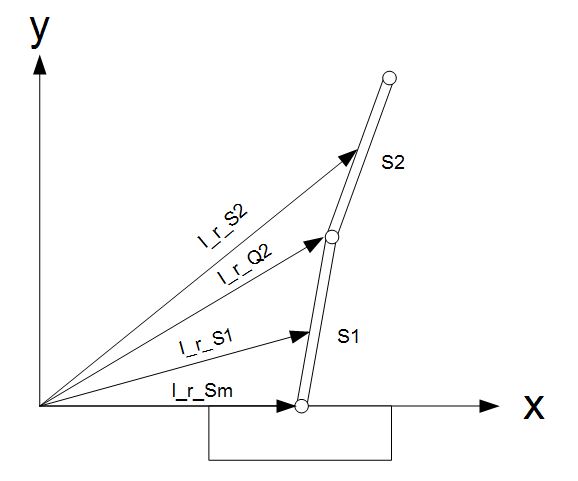
\includegraphics[width=10cm]{Ortsvektoren}}
\caption{Ortsvektoren zu den Gelenk- und Schwerpunkten}
\end{figure}
\begin{lstlisting}
%---- Drehmatrix Stab 1
T_IK1 = [cos(th1) sin(th1) 0;
        -sin(th1) cos(th1) 0;
          0          0     1];
%---- Drehmatrix Stab 2
T_IK2 = [cos(th2) sin(th2) 0;
        -sin(th2) cos(th2) 0;
          0          0     1];

%---- Ortsvektoren
I_r_Sm = [x;0;0];
I_r_S1 = [x+l1/2*sin(th1) ; l1/2*cos(th1) ; 0];
I_r_Q2 = [x+l1*sin(th1) ; l1*cos(th1) ; 0];
K1_r_Q1S1 = [0; l1/2; 0];
K2_r_Q2S2 = [0; l2/2; 0];
I_r_S2 = I_r_Q2 + T_IK2 * K2_r_Q2S2;

%---- Traegheitstensoren in den koerperfesten Koordinatensystemen
K1_I_S1 = diag([0 0 I_1]);
K2_I_S2 = diag([0 0 I_2]);

%---- Winkelgeschwindigkeitsvektoren der Staebe
K_om1 = [0 ; 0 ; -th1_p];
K_om2 = [0 ; 0 ; -th2_p];

%---- JACOBI-Matrizen der Translation
J_Tm = jacobian(I_r_Sm, q);
J_T1 = jacobian(I_r_S1, q);
J_T2 = jacobian(I_r_S2, q);

%---- JACOBI-Matrizen der Rotation
J_R1 = jacobian(K_om1, q_p);
J_R2 = jacobian(K_om2, q_p);

%---- Geschwindigkeitsvektoren
I_v_Sm = J_Tm*q_p ;
I_v_S1 = J_T1*q_p ; 
I_v_S2 = J_T2*q_p ;

%---- kinetische Energie
T = 1/2*(mm*(I_v_Sm.'*I_v_Sm)+m1*(I_v_S1.'*I_v_S1)
		+m2*(I_v_S2.'*I_v_S2)+K_om1.'*K1_I_S1*K_om1
		+K_om2.'*K2_I_S2*K_om2);        
T = simplify(T);

%---- potentielle Energie
V=-(m1*I_r_S1.'+m2*I_r_S2.')*[0 ; -g ; 0];

%---- Ableitungen fuer LAGRANGEsche Gleichung 2. Art
dTdv = simplify(jacobian(T,q_p).');
dTdq = simplify(jacobian(T,q).');
dVdq = simplify(jacobian(V,q).');

%---- Elemente der Bewegungsgleichung M(q)*q_pp + f(q,q_p) = 0
M = simplify(jacobian(dTdv,q_p));
f = simplify(jacobian(dTdv,q)*q_p+dVdq-dTdq-[F;0;0]);

%=============================================================
%---- Linearisierung um die Gleichgewichtslage:
%     th1 = 0, th2 = 0, x = 0
M0 = subs(M,{th1, th2, x},{0, 0, 0});
f0 = subs(f,{x, th1, th2, x_p, ...
    th1_p, th2_p},{0, 0, 0, 0, 0, 0});
    
%Auslenkungs-proportionaler Anteil
Q = subs(jacobian(f,q),{x, th1, th2, x_p, ...
    th1_p, th2_p},{0, 0, 0, 0, 0, 0});
    
%Gesschwindigkeits-proportionaler Anteil
P = subs(jacobian(f,q_p),{x, th1, th2, x_p, ...
    th1_p, th2_p},{0, 0, 0, 0, 0, 0});
\end{lstlisting}

\section{Zustandsraumdarstellung und Reglerentwurf}
Um die Auslegung des LQ-Reglers effizient gestalten zu können transformieren wir unser Problem in den Zustandsraum. Wir berechnen zunächst die benötigten Matrizen. Durch ersetzen der symbolischen Variablen durch ihre Zahlenwerte, kann das System numerisch verarbeitet werden. Mit dem Befehl lqr() lassen sich in Matlab aus den systembeschreibenden Matrizen, die Rückkopplungsparameter für eine LQ-Regelung berechnen. Der Befehl ss() konvertiert unser System nach Festlegung der Ein- und Augänge in den Zustandsraum. Schließlich erfolgt die Simulation mit der gewünschten Simulationsdauer und des konstanten Offsets.

\begin{lstlisting}
%----Erstellen und Simulieren der Zustandsraumdarstellung

A = [zeros(3),eye(3);
    -M0^(-1)*Q, -M0^(-1)*P];
A = double(subs(A,{mm, m1, m2, l1, l2, g, I_1, I_2}, ...
    {0.2, 0.01, 0.01, 0.5, 0.7, 9.81, 2.0833e-04, 4.0833e-04}));
A(7,7) = 0;
A(7,1) = -1

B = [zeros(3,1);M0^(-1)*[1;0;0]];
B = double(subs(B,{mm, m1, m2, l1, l2, g, I_1, I_2}, ...
    {0.2, 0.01, 0.01, 0.5, 0.7, 9.81, 2.0833e-04, 4.0833e-04}));
B(7,1) = 0
Bxc = [0; 0; 0; 0; 0; 0; 1]

C = [1 0 0 0 0 0 0;
   0 1 0 0 0 0 0;
   0 0 1 0 0 0 0]

D = [0; 0; 0]

%Gewichtungsmatrix und Gewichtungsfaktor
Q=eye(7);
r=1;

%----lqr Regelungsentwurf
k = lqr(A,B,Q,r)

%----neue Zustandsraumsystemmatrizen nach Parameterruekfuehrung
Ac = [(A-B*k)];
Bc = [Bxc];
Cc = [C];
Dc = [D];

states = {'x' 'th1' 'th2' 'x_p' 'th1_p' 'th2_p' 'in'};
inputs = {'F'};
outputs = {'x' 'th1' 'th2'};

sys_cl = ss(Ac,Bc,Cc,Dc,'statename',states,'inputname',inputs,'outputname',outputs);

%----definieren des Simulationszeitraums
t = 0:0.01:8;

%----definition des konstanten 0.2m offsets als Input
u =0.2*ones(size(t));

%----Simulation des erstellten Systems ueber gegebene Zeit mit bekanntem
%Input
[y,t,x]=lsim(sys_cl,u,t);
\end{lstlisting}
Die Form der Zustandsraumdartsellung, mit den Matrizen $A_{c}$ und $B_{c}$ siehe Abbildung(3.2), sieht folgendermaßen aus:\\\\
\begin{equation}
\label{eqn:Zustandraumdarstellung}
\mathbf{\dot{x}}=A_{c} \mathbf{x}+B_{c} u 
\end{equation}
\begin{equation}
\mathbf{y}=C_{c} \mathbf{x}+D_{c} u
\end{equation}
\\
Mit den zugehörigen numerischen Werten ergibt sich:
\\ \\
\begin{equation*}
\begin{bmatrix}
\dot{x} \\
\dot{\theta_{1}}\\
\dot{\theta_{2}}\\
\ddot{x}\\
\ddot{\theta_{1}}\\
\ddot{\theta_{2}}\\
i_{n}\\
\end{bmatrix}
=
\begin{bmatrix}
0 & 0 & 0 & 1 & 0 & 0 & 0\\
0 & 0 & 0 & 0 & 1 & 0 & 0\\
0 & 0 & 0 & 0 & 0 & 1 & 0\\
-13.6504 & 161.0731 & -255.2710 & -16.4349 & -1.8996 & -41.5292 & 4.9296\\
35.1012 & -363.7374 & 631.1872 & 42.2612 & 4.8846 & 106.7898 & -12.6761\\
-8.3575 & 44.5622 & -108.2415 & -10.0623 & -1.1630 & -25.4264 & 3.0182\\
-1 & 0 & 0 & 0 & 0 & 0 & 0\\
\end{bmatrix}
\begin{bmatrix}
x \\
\theta_{1}\\
\theta_{2}\\
\dot{x}\\
\dot{\theta_{1}}\\
\dot{\theta_{2}}\\
e\\
\end{bmatrix}
+
\begin{bmatrix}
0\\
0\\
0\\
0\\
0\\
0\\
1\\
\end{bmatrix}
F
\end{equation*}


\begin{equation*}
\begin{bmatrix}
x\\
\theta_{1}\\
\theta_{2}\\
\end{bmatrix}
=
\begin{bmatrix}
1 & 0 & 0 & 0 & 0 & 0 \\
0 & 1 & 0 & 0 & 0 & 0 \\
0 & 0 & 1 & 0 & 0 & 0 \\
\end{bmatrix}
\begin{bmatrix}
x \\
\theta_{1}\\
\theta_{2}\\
\dot{x}\\
\dot{\theta_{1}}\\
\dot{\theta_{2}}\\
e\\
\end{bmatrix}
+
\begin{bmatrix}
0 \\
0 \\
0 \\
\end{bmatrix}
F
\end{equation*}

\section{Simulation und Ausgabe}
Um die Ergebnisse besser interpretieren zu können wurden die Position $x$, sowie die zwei Winkel $\theta_{1}$ und $\theta_{2}$ in Abbildung 4.3 über die Zeit geplottet. Zudem werden noch die Eigenwerte berechnet und ausgegeben.  
\begin{lstlisting}
%----Drei einzelne Diagramme in einem Fenster
figure(1);
ax(1) = subplot(3,1,1);
    plot(ax(1),t,y(:,1),'b');
    title(ax(1),'cart position'); 
    ylim([-0.1,0.25]);            
    grid on                       
ax(2) = subplot(3,1,2);           
    plot(ax(2),t,y(:,2),'r');     
    title(ax(2),'angle th 1');
    grid on
ax(3) = subplot(3,1,3);
    plot(ax(3),t,y(:,3),'g');
    title(ax(3),'angle th 2');
    grid on

%----Berechnung der Eigenwerte
Eigenwerte = eig(Ac)
\end{lstlisting}
Wie sich in der Ausgabe erkennen lässt sind die Realteile aller Eigenwerte negativ. Somit ist das betrachtete System stabil!
\begin{figure}[h]
\centering  %Zentrierung
{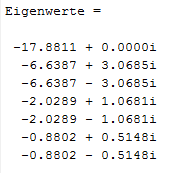
\includegraphics[width=5cm]{Eigenwerte}}
\caption{Ausgabe der Eigenwerte}
\end{figure}

\begin{figure}[h]
\centering  %Zentrierung
{\includegraphics[width=15cm]{AusgabeMATLAB}}
\caption{MATLAB Plot}
\end{figure}

%\renewcommand{\thechapter}{}
\chapter{Implementierung in MalpeSim}
%\renewcommand{\thechapter}{4}
Nachdem das vorherige Kapitel ausschließlich der Implementierung in MATLAB gewidment wurde, beschäftigt sich dieses nun mit der Umsetzung mittels einer \textit{nicht klassischen}, blockorientierten, grafischen Programmierung in MapleSim. \\
Zuerst wird das Modell (in unserem Fall das geregelte mechanische Doppelpendel) im MapleSim GUI nachgebildet. Anschließend können Signale direkt an diesem Model abgegriffen und ins System rückgeführt werden. Dadurch lassen sich selbst komplexe dynamische Systeme aus allen Bereichen der Natur- und Ingeneurswissenschaften vergleichsweise einfach modellieren.
\section{Modellbildung}
Da hier keine mathematischen Transformationen mehr nötig sind um das Doppelpendel in MapleSim modellieren zu können, werden die Größen aus der Angabe direkt verwendet. Die Materialparamter sind selbstverständlich die, die auch schon in den anderen Kapiteln verwendet wurden. \\
\begin{figure}[h]
\centering  %Zentrierung
\label{MapleSimModell}
{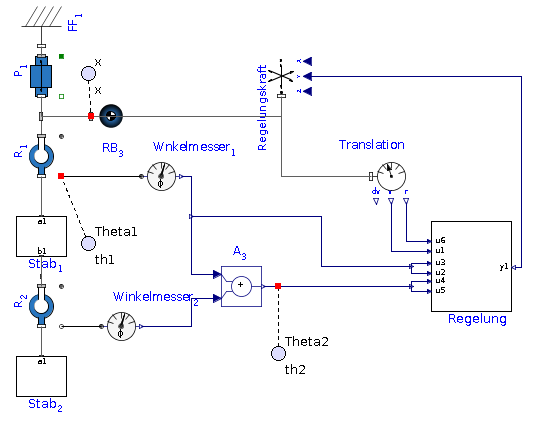
\includegraphics[width=\textwidth]{MapleSimModel}}
\caption{Modell in MapleSim}
\end{figure}
\newpage \noindent
Das Pendel wurde aus Komponenten der \textit{Multibody}-Bibliothek aufgebaut. Es besteht aus einem festen Rahmen (\textit{fixed frame}), zwei Drehgelenken (\textit{revolutes}), einem Schlitten (\textit{prismatic}) und den zwei Stäben. \\
Da es innerhalb der Standardbibliotheken keine Kompnenten gab, die die geforderten mechanischen Eigenschaften erfüllen, wurden die Stäbe aus jeweils zwei starren Körpern (\textit{rigid body frames}) und einer Punktmasse (\textit{point mass}) nachgebildet. Die Komponenten der Stäbe wurden aus Gründen der Übersichtlichkeit zu Subsystemen zusammengefasst. Selbstverständlich sind die Eigenschaften (Abmessungen, Tägheitstensoren und Schwerpunktsabstände) der nachgebildeten Stäbe identisch zu jenen aus der Angabe.
\section{Regelung}
Auch der Bau des Reglers ist vergleichweise einfach. Die nötigen Zustandsgrößen $\theta_{1}$, $\theta_{2}$ und $x$ können direkt abgegriffen und weiterverwendet werden. \\
$\theta_{1}$ wird dabei unverändert dem Regelungssubsystem übergeben. Für $\theta_{2}$ wird der Winkel, den die beiden Stäbe miteinander einschließen, gemessen und zu $\theta_{1}$ addiert. Der Abstand des Schlittens vom Ursprung des Koordinatensystems $x$ kann auch direkt ausgelesen und weitergeben werden. 
Wie schon bei den Stäben wurde die Regelung zu einem Subsystem zusammengefasst um eine hohe Übersicht gewährleisten zu können. Dieser Regelung möchten wir uns nun widmen. \newpage
\begin{figure}
\centering  %Zentrierung
\label{SubsystemRegelung}
{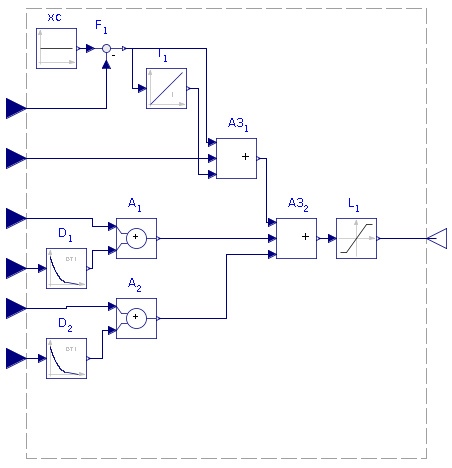
\includegraphics[width=7cm]{MapleSimRegelungCut}}
\caption{Subsystem Regelung}
\end{figure}
\noindent
Wie der Angabe zu entnehmen ist, bedarf es einer Regelung um das instabile System im Gleichgewicht zu halten. Dabei wird die Kraft als Regelung in Form einer Zustandsrückführung, kombiniert mit einer Positionsregelung der Form
\begin{equation}
\label{Auslenkungen}
e = x_{e} - x \qquad \dot{e} = - \dot{x} \qquad i_{in} = \int_{t_{0}}^{t_{end}} e  dt,
\end{equation}
angesetzt:
\begin{equation}
\label{Rueckstellkraft}
F = k_{x}e + k_{\dot{x}}\dot{x} + k_{in}i_{in} + k_{\theta_{1}}\theta_{1} + k_{\theta_{2}}\theta_{2} + k_{\dot{\theta}_{1}}\dot{\theta}_{1} + k_{\dot{\theta}_{2}}\dot{\theta}_{2}
\end{equation}
Nach Gleichung \ref{Rueckstellkraft} ist die Rückstellkraft also eine Linearkombination der Winkel und ihren zeitlichen Ableitungen, sowie einer
momentanen Auslenkungsdifferenz des Schlittens vom Sollwert, mit der zugehörigen zeitlichen Ableitung und dem zeitlichen Integral [über besagte Auslenkung]. \\ \\
Wie sich in Abbildung \ref{MapleSimModell} erkennen lässt werden die Winkel jeweils doppelt übergeben. Intern wird dann jeweils ein Signal dieser Signalpaare differenziert. Anschließend werden die Signale mit den zugehörigen Rückkopplungparametern $k_{\theta_{1}}$ und $k_{\theta_{2}}$ beziehungsweise $k_{\dot{\theta}_{1}}$ und $k_{\dot{\theta}_{2}}$ in den Addierern $A_{1}$ und $A_{2}$ aufsummiert. \\
Ein ähnliches Prodzedere ergibt sich auch für die anderen beiden Eingänge $x$ und  $\dot{x}$. Mit der Auslenkung $x$ wird nach den Gleichungen \ref{Auslenkungen} die Abweichung $e$ vom Sollzustand $x_{e}$ berechnet, welche anschließend im Integrationsglied $I_{1}$ integriert wird. Auch hier werden die Paramter wieder mit den zugehörigen Koeffizienten $k_{x}$, $k_{\dot{x}}$ und $k_{in}$ gewichtet und anschließend in den Addierern $A3_{1}$ und $A3_{2}$ summiert. \\
Da die Rückstellkraft nicht unendlich groß werden darf wurde abschließend noch eine Kraftbegrenzung $L_{1}$ hinzugefügt, welche die Rückstellkraft $F$ auf maximal 10 [N] beschränkt. \\
Damit ist die Regelung abgeschlossen und die Kraft wird am Ausgang $y1$ (Siehe Abbildung \ref{MapleSimModell}) ausgegeben und mit dem Element \textit{applied world force} in das mechanische System rückgeführt. \\
Um die Zuordnung innerhalb des Regelungssubsystems zu vereinfachen wurde noch eine Korrespondenztabelle erstellt. Die Eingänge werden (nach Abbildung \ref{SubsystemRegelung}) von oben nach unten aufgezählt. \\ \\
\center
\begin{tabular}{ l | c | r }
 	Nummer & Bezeichnung Global & Größe \\	
	\hline
  	1 & u6 & $x$ \\
  	2 & u1 & $\dot{x}$ \\
  	3 & u3 & $\theta_{1}$ \\
  	4 & u2 & $\theta_{1}$ \\
  	5 & u4 & $\theta_{2}$ \\
  	6 & u5 & $\theta_{2}$ \\
	\hline
	7 & y1 & F
\end{tabular}

\chapter{Zusammenfassung}

\end{document}
